% =============================================================================
% CHƯƠNG 4 — PHÁT TRIỂN ỨNG DỤNG MARKETING COMMAND CENTER VÀ KHAI THÁC DỮ LIỆU
% Nội dung đối chiếu với repo marketpulse-360 @ dbe614b và docs/runbooks/story-demo.md.
% =============================================================================

Dữ liệu chỉ tạo ra giá trị khi đến được tay người ra quyết định. Chương này trình bày cách MarketPulse 360 đưa kết quả của đường ống tới người dùng qua ứng dụng \emph{Marketing Command Center}: kiến trúc phục vụ, thiết kế cơ sở dữ liệu vận hành, và kết quả khai thác thực tế cho từng yêu cầu nghiệp vụ trên bộ dữ liệu story-demo.

\section{Kiến trúc ứng dụng}
\label{sec:c4-kien-truc}

Ứng dụng gồm giao diện Next.js~\cite{nextjsdocs}, một proxy nội bộ và tầng API FastAPI~\cite{fastapidocs} (Hình~\ref{fig:app-architecture}). Trình duyệt không bao giờ gọi thẳng vào API: mọi lời gọi đi qua route \texttt{/api/v1/*} của Next.js, nơi chỉ chuyển tiếp cookie phiên, header \texttt{Origin} và kiểu nội dung. FastAPI chịu trách nhiệm xác thực, phân quyền và truy vấn ba nhóm kho dữ liệu tách biệt.

\begin{figure}[H]
    \centering
    \resizebox{\textwidth}{!}{\input{chapters/Figs/fig-app-architecture}}
    \caption{Kiến trúc tầng phục vụ ứng dụng Marketing Command Center}
    \label{fig:app-architecture}
\end{figure}

\subsection{API FastAPI và ghim phiên bản đọc}
\label{sec:c4-api}
Tầng API cung cấp 41 route, gồm các nhóm bảng điều khiển, phân tích hành trình, vòng đời khách hàng, insight, vận hành và xác thực. Mỗi request đọc số liệu đã kiểm chứng đều \emph{ghim} một bản phát hành: API tra \texttt{publication\_journal} lấy bản có \texttt{generation} lớn nhất, rồi dùng đúng CSDL \texttt{mp\_release\_*} của bản đó cho mọi truy vấn trong request. Nhờ vậy, nếu một bản phát hành mới được công bố giữa chừng, người dùng vẫn nhận được kết quả nhất quán từ một bản duy nhất. Mọi phản hồi đều kèm thông tin nguồn gốc (mã release, ngày dữ liệu) để giao diện hiển thị độ tươi của số liệu. Số tiền được truyền dưới dạng chuỗi số nguyên để tránh sai số dấu phẩy động.

\subsection{Tiến trình nền cho dữ liệu trực tiếp}
\label{sec:c4-workers}
Ba tiến trình nền bổ sung dữ liệu cho ứng dụng. \texttt{campaign-worker} đọc topic \texttt{marketing.gold.campaign-metrics.v1} và nạp vào \texttt{marketpulse\_live.campaign\_snapshots}; \texttt{live-events-worker} đọc \texttt{marketing.clean.customer-events.v1} và nạp vào \texttt{marketpulse\_live.events}. Cả hai dùng chế độ \texttt{read\_committed} và commit offset thủ công sau khi ghi thành công, nên một lần gửi lại chỉ trùng về vị trí và được loại theo khóa \texttt{(partition, offset)}. Tiến trình \texttt{journey-publish} chạy một lần cho mỗi release: nó đọc \texttt{silver.customer\_events} tại đúng snapshot đã ghim, chỉ giữ sự kiện có đồng thuận và không thuộc phiên bot, thay \texttt{profile\_key} bằng bút danh \texttt{profile\_ref} rồi ghi vào CSDL sidecar \texttt{mp\_journey\_*}.

\subsection{Xác thực, phân quyền và kiểm toán}
\label{sec:c4-rbac}
Ứng dụng không có tài khoản mặc định và không có công tắc tắt xác thực. Tài khoản do quản trị viên tạo bằng dòng lệnh; mật khẩu chỉ được lưu dưới dạng băm scrypt có salt ngẫu nhiên. Khi đăng nhập, máy chủ cấp một token ngẫu nhiên 32 byte trong cookie \texttt{HttpOnly}, \texttt{SameSite=Strict}; cơ sở dữ liệu chỉ lưu SHA-256 của token, với thời hạn tuyệt đối 8 giờ. Đăng nhập sai quá 5 lần trong 15 phút sẽ bị chặn tạm thời. Ba vai trò được phân cấp rõ ràng:

\begin{itemize}
    \item \texttt{viewer}: xem các bảng điều khiển tổng hợp, phễu, phân bổ, cohort, cảnh báo và mô phỏng chỉ đọc;
    \item \texttt{operator}: thêm quyền xem hồ sơ và dòng thời gian khách hàng, tạo phân đoạn, sửa ngân sách và quy tắc cảnh báo;
    \item \texttt{admin}: thêm quyền xem sức khỏe hệ thống, chạy kiểm chứng chất lượng và quản lý tài khoản.
\end{itemize}

Kiểm tra quyền diễn ra ở máy chủ \emph{trước} mọi truy vấn dữ liệu. Mọi quyết định truy cập được ghi vào bảng \texttt{access\_audit} chỉ cho phép thêm mới; một trigger sẽ từ chối mọi lệnh \texttt{UPDATE} và \texttt{DELETE}.

\section{Cơ sở dữ liệu vận hành}
\label{sec:c4-csdl-van-hanh}

Dữ liệu do người dùng ứng dụng tạo ra (tài khoản, cấu hình, quy tắc, phân đoạn) có bản chất giao dịch: cần ràng buộc chặt, cập nhật có kiểm soát phiên bản và nhật ký bất biến. Phần này vì vậy được đặt trên PostgreSQL 17.6~\cite{postgresdocs}, tách hẳn khỏi kho phân tích.

\subsection{Lược đồ marketpulse\_app (PostgreSQL)}
\label{sec:c4-pg-app}
Lược đồ \texttt{marketpulse\_app} có 12 bảng, chia thành bốn nhóm (Hình~\ref{fig:schema-postgres} và Hình~\ref{fig:schema-postgres-2}):

\begin{itemize}
    \item \textbf{Bảo mật:} \texttt{auth\_users}, \texttt{auth\_sessions} (khóa ngoại tới người dùng), \texttt{login\_failures} (bộ đếm theo cửa sổ 15 phút) và \texttt{access\_audit} (nhật ký bất biến).
    \item \textbf{Phân đoạn khách hàng:} \texttt{segments} giữ phiên bản hiện hành, mỗi lần sửa sinh một dòng mới trong \texttt{segment\_revisions} (khóa chính kép \texttt{(segment\_id, version)}, bất biến nhờ trigger). Phân đoạn và phiên bản đầu tiên được ghi trong cùng một giao dịch, nên mỗi phân đoạn luôn có ít nhất một phiên bản.
    \item \textbf{Ngân sách và cảnh báo:} \texttt{campaign\_settings}, \texttt{alert\_rules}, \texttt{alert\_evaluations} và \texttt{alert\_occurrences}. Khóa \texttt{evaluation\_key} là SHA-256 của quy tắc, phiên bản, cửa sổ thời gian và release, nên một lần đánh giá chạy lại không tạo cảnh báo trùng.
    \item \textbf{Vận hành:} \texttt{quality\_reports} lưu kết quả kiểm chứng (bất biến) và \texttt{ops\_state} là bảng một dòng.
\end{itemize}

Đáng chú ý, \texttt{campaign\_id} trong cấu hình và quy tắc cảnh báo \emph{không} là khóa ngoại: chiến dịch nằm trong kho phân tích ClickHouse, nên API kiểm tra chiến dịch có tồn tại trong release đang phục vụ trước khi ghi. Các thao tác ghi dùng khóa lạc quan theo cột \texttt{version} để hai người cùng sửa không ghi đè lẫn nhau.

\subsection{Lược đồ marketpulse\_ops (PostgreSQL)}
\label{sec:c4-pg-ops}
Lược đồ \texttt{marketpulse\_ops} nằm trên một instance PostgreSQL riêng của khối batch và gồm 4 bảng sổ cái của quy trình công bố. \texttt{preparations} lưu phiếu chuẩn bị bất biến; \texttt{publications} và \texttt{certified\_bundles} có quan hệ 1--0..1 với \texttt{preparations} qua khóa ngoại thật; \texttt{attempts} đếm số lần thử theo giai đoạn và được tham chiếu mềm, vì lần thử đầu tiên được cấp \emph{trước} khi phiếu chuẩn bị tồn tại.

\begin{figure}[!htbp]
    \centering
    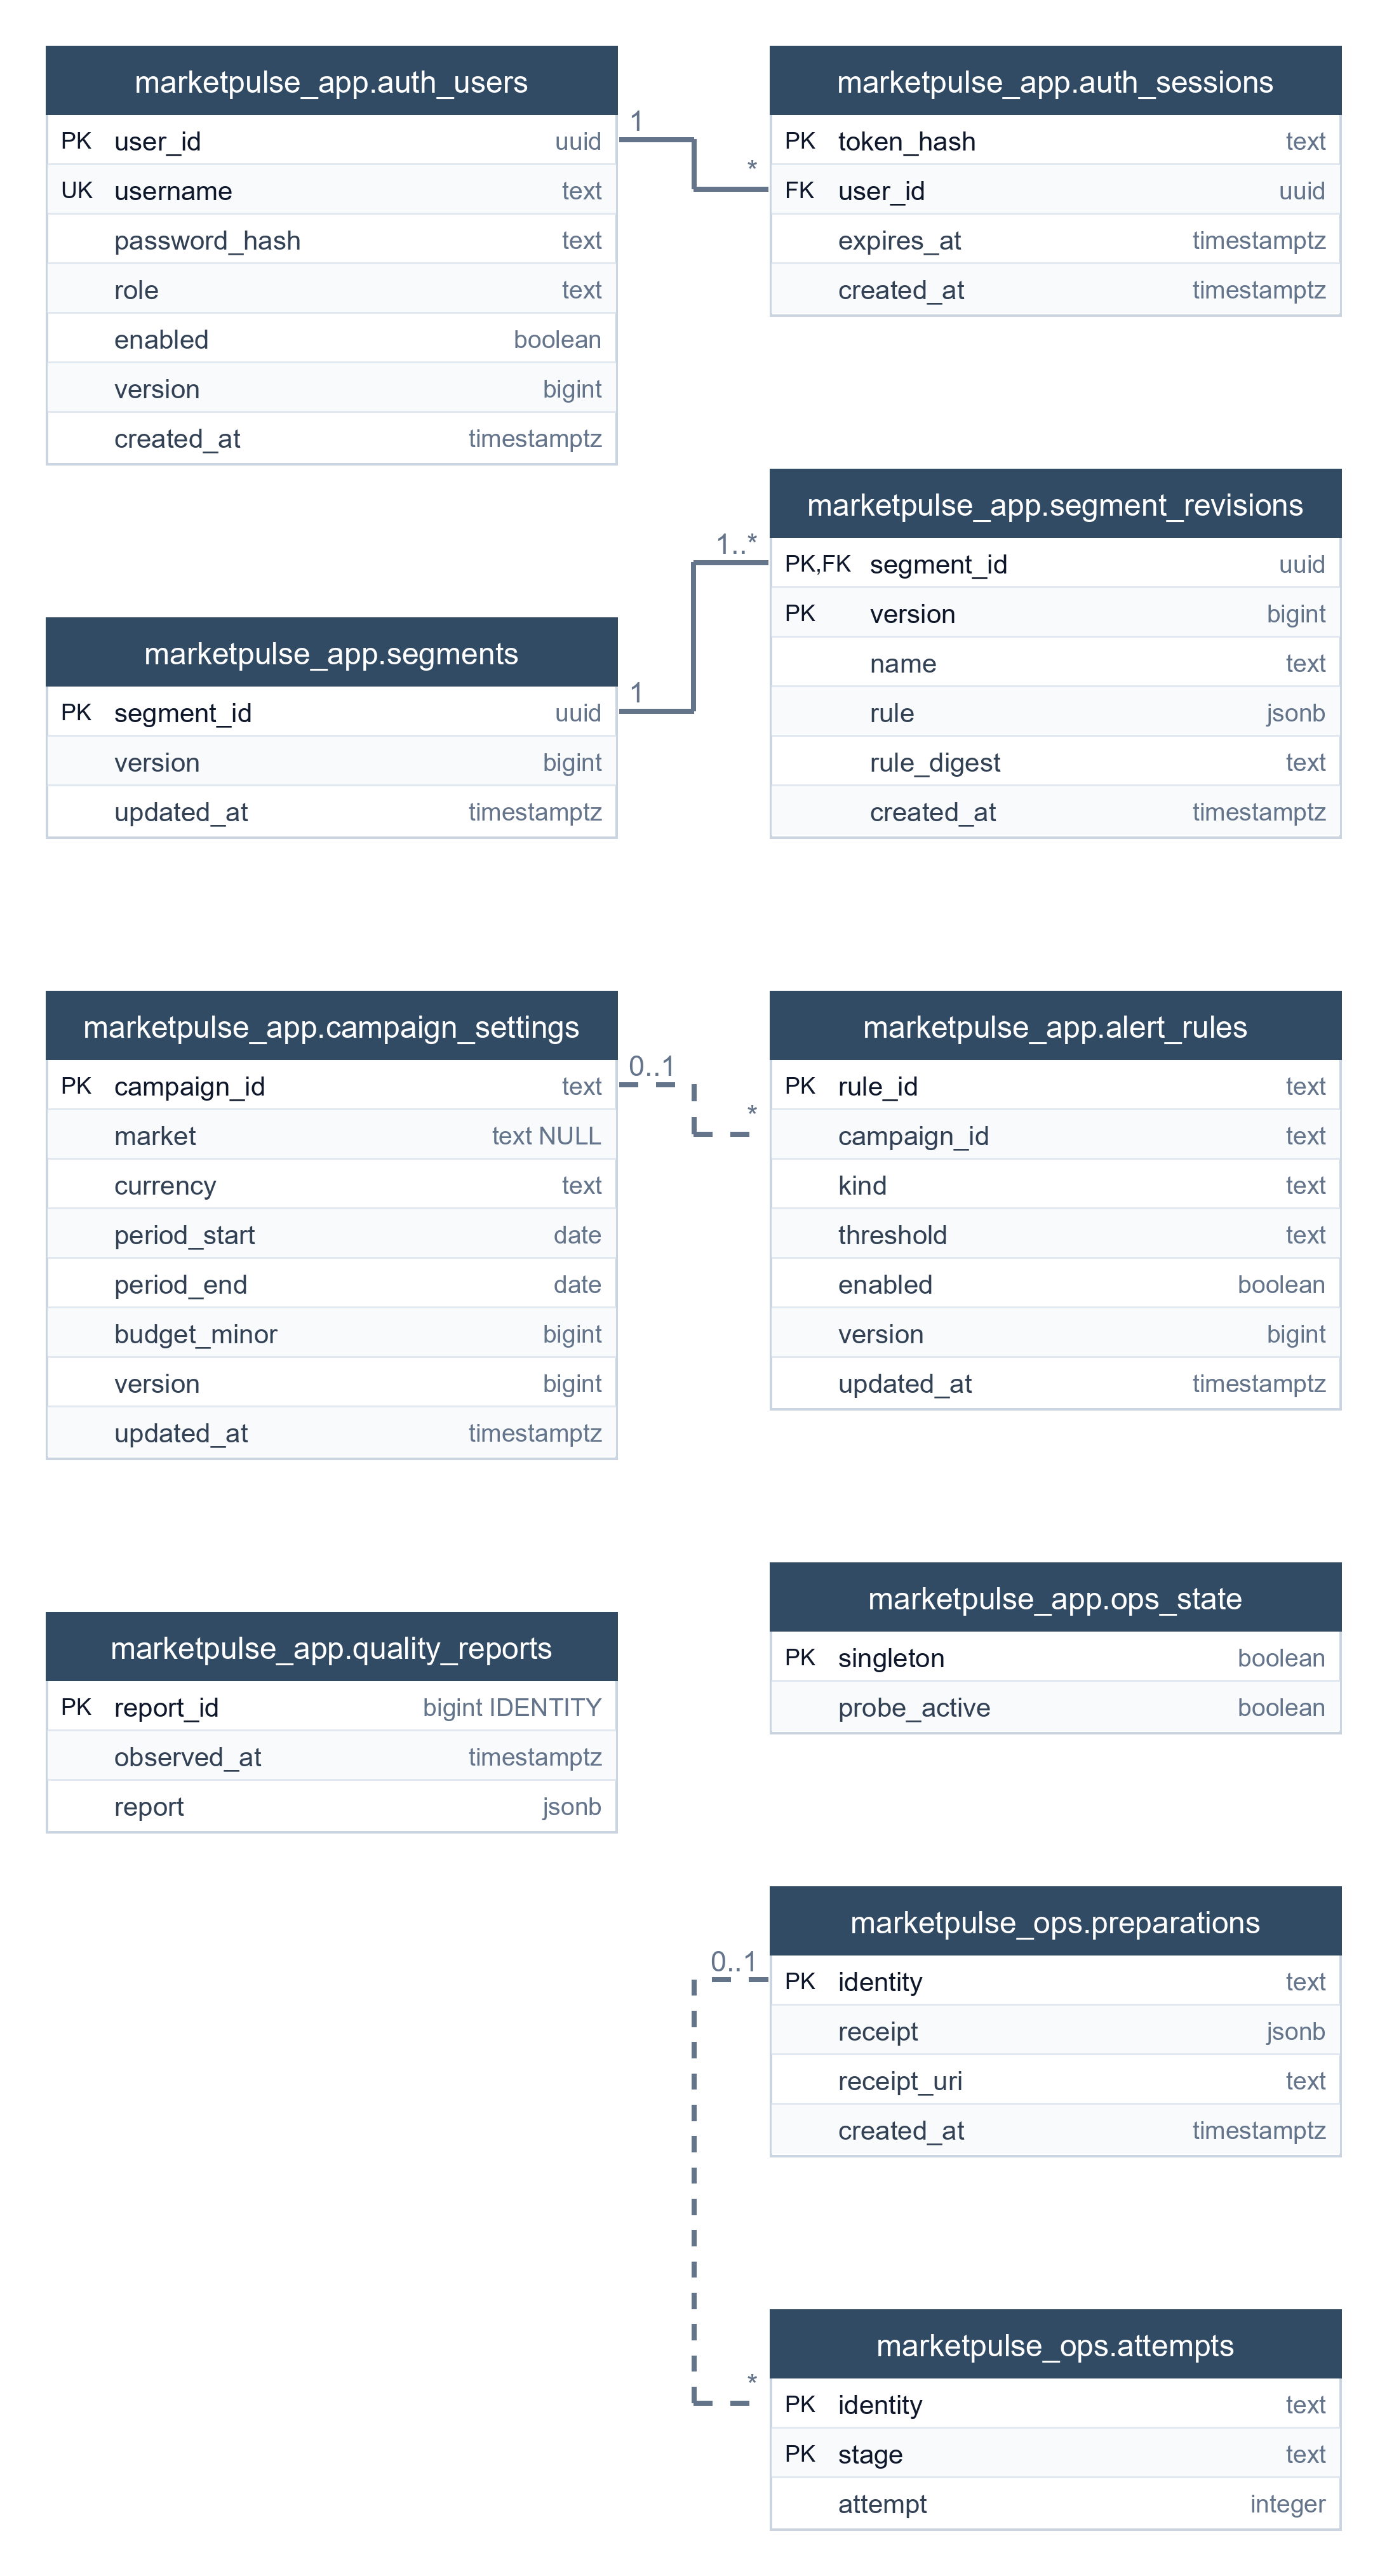
\includegraphics[width=\textwidth, height=0.88\textheight, keepaspectratio]{chapters/Pics/schema-postgres-1.png}
    \caption{Lược đồ quan hệ PostgreSQL (phần 1): tài khoản, phân đoạn, cấu hình chiến dịch, quy tắc cảnh báo và chuẩn bị công bố}
    \label{fig:schema-postgres}
\end{figure}

\begin{figure}[!htbp]
    \centering
    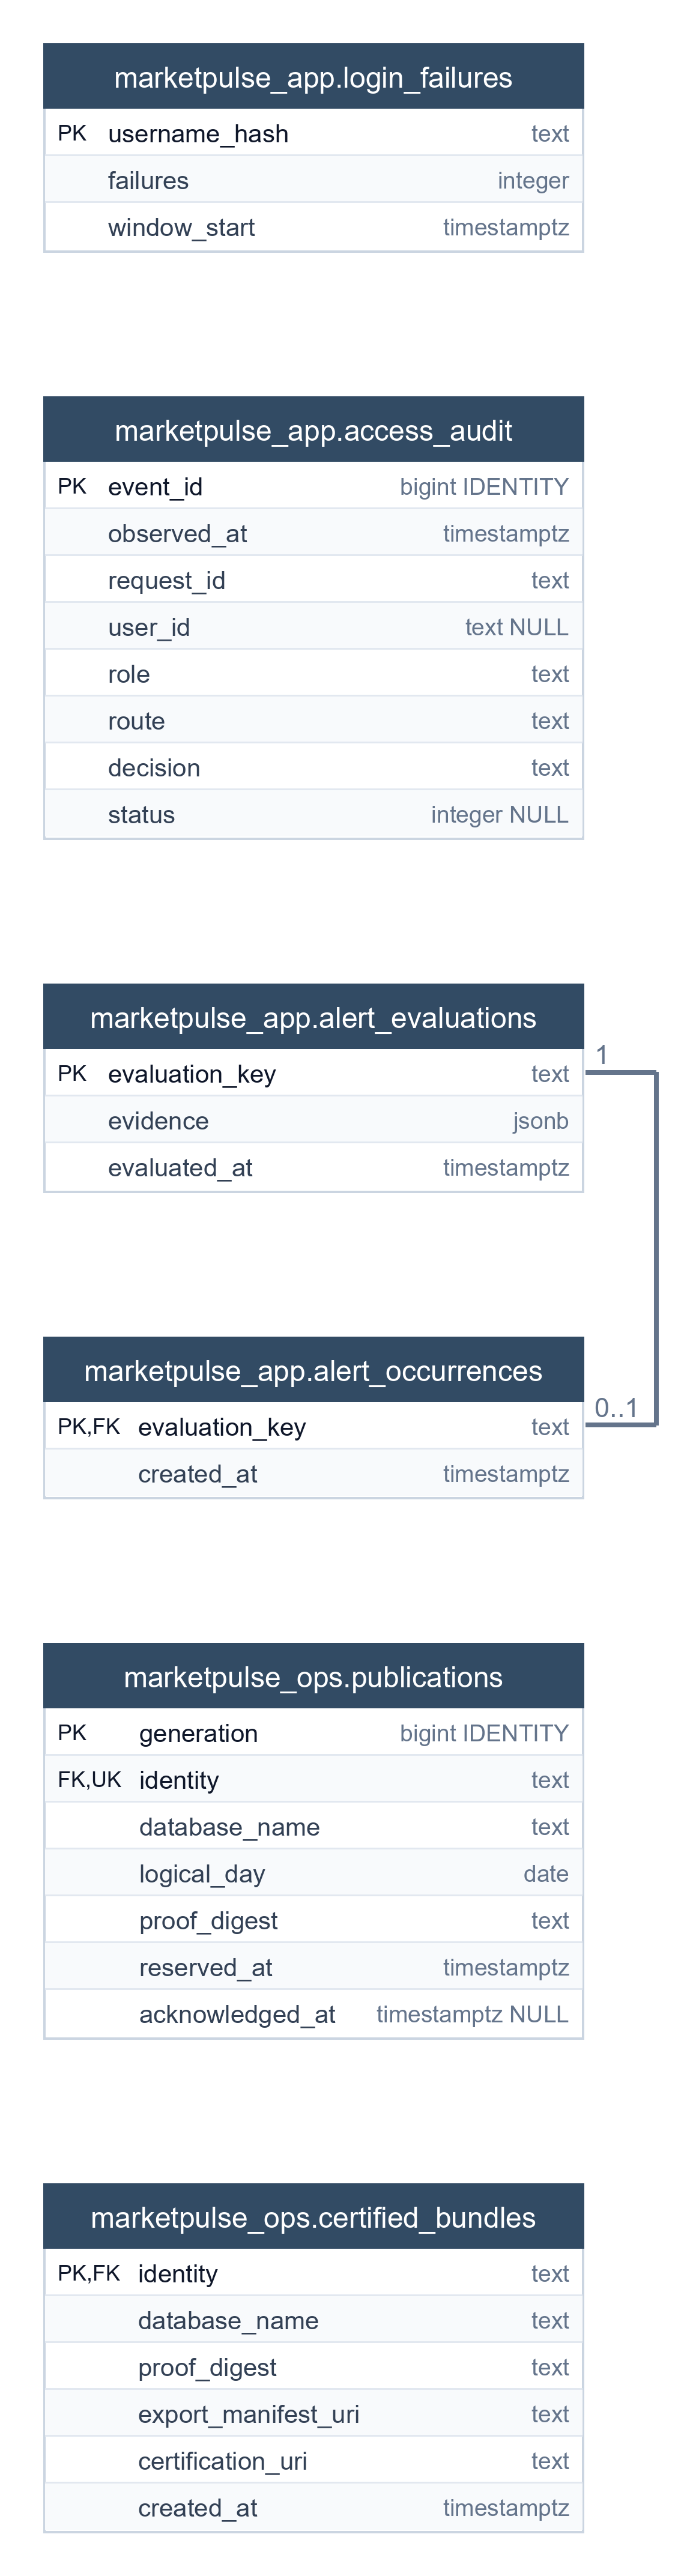
\includegraphics[width=\textwidth, height=0.88\textheight, keepaspectratio]{chapters/Pics/schema-postgres-2.png}
    \caption[Lược đồ quan hệ PostgreSQL (phần 2): kiểm toán truy cập, kết quả cảnh báo và sổ cái công bố]{Lược đồ quan hệ PostgreSQL (phần 2): kiểm toán truy cập, kết quả cảnh báo và sổ cái công bố. Khóa ngoại sang phần 1: \texttt{alert\_evaluations} tới \texttt{alert\_rules}; \texttt{publications} và \texttt{certified\_bundles} tới \texttt{preparations}}
    \label{fig:schema-postgres-2}
\end{figure}

\subsection{Các bảng phục vụ trên ClickHouse}
\label{sec:c4-clickhouse}
Ngoài các CSDL release, ClickHouse còn chứa ba nhóm bảng phục vụ ứng dụng (Hình~\ref{fig:schema-clickhouse} và Hình~\ref{fig:schema-clickhouse-2}). \texttt{marketpulse\_serving.publication\_journal} là nhật ký chỉ ghi thêm, phản chiếu bảng \texttt{publications} của sổ cái; \texttt{journey\_publications} ghi nhận CSDL hành trình của từng release. Trong CSDL sidecar, bảng \texttt{events} lưu hành trình đã ẩn danh và view \texttt{paid\_touches} chọn click trả phí đầu tiên cho mỗi cặp \texttt{(profile\_ref, click\_id)}. Kho \texttt{marketpulse\_live} gồm \texttt{campaign\_snapshots} (MergeTree), \texttt{events} (ReplacingMergeTree theo \texttt{(partition, offset)}) và hai bảng một dòng ghim định danh nguồn Kafka: nếu cụm Kafka hoặc topic bị thay đổi, worker từ chối ghi thay vì trộn hai nguồn.

\begin{figure}[!htbp]
    \centering
    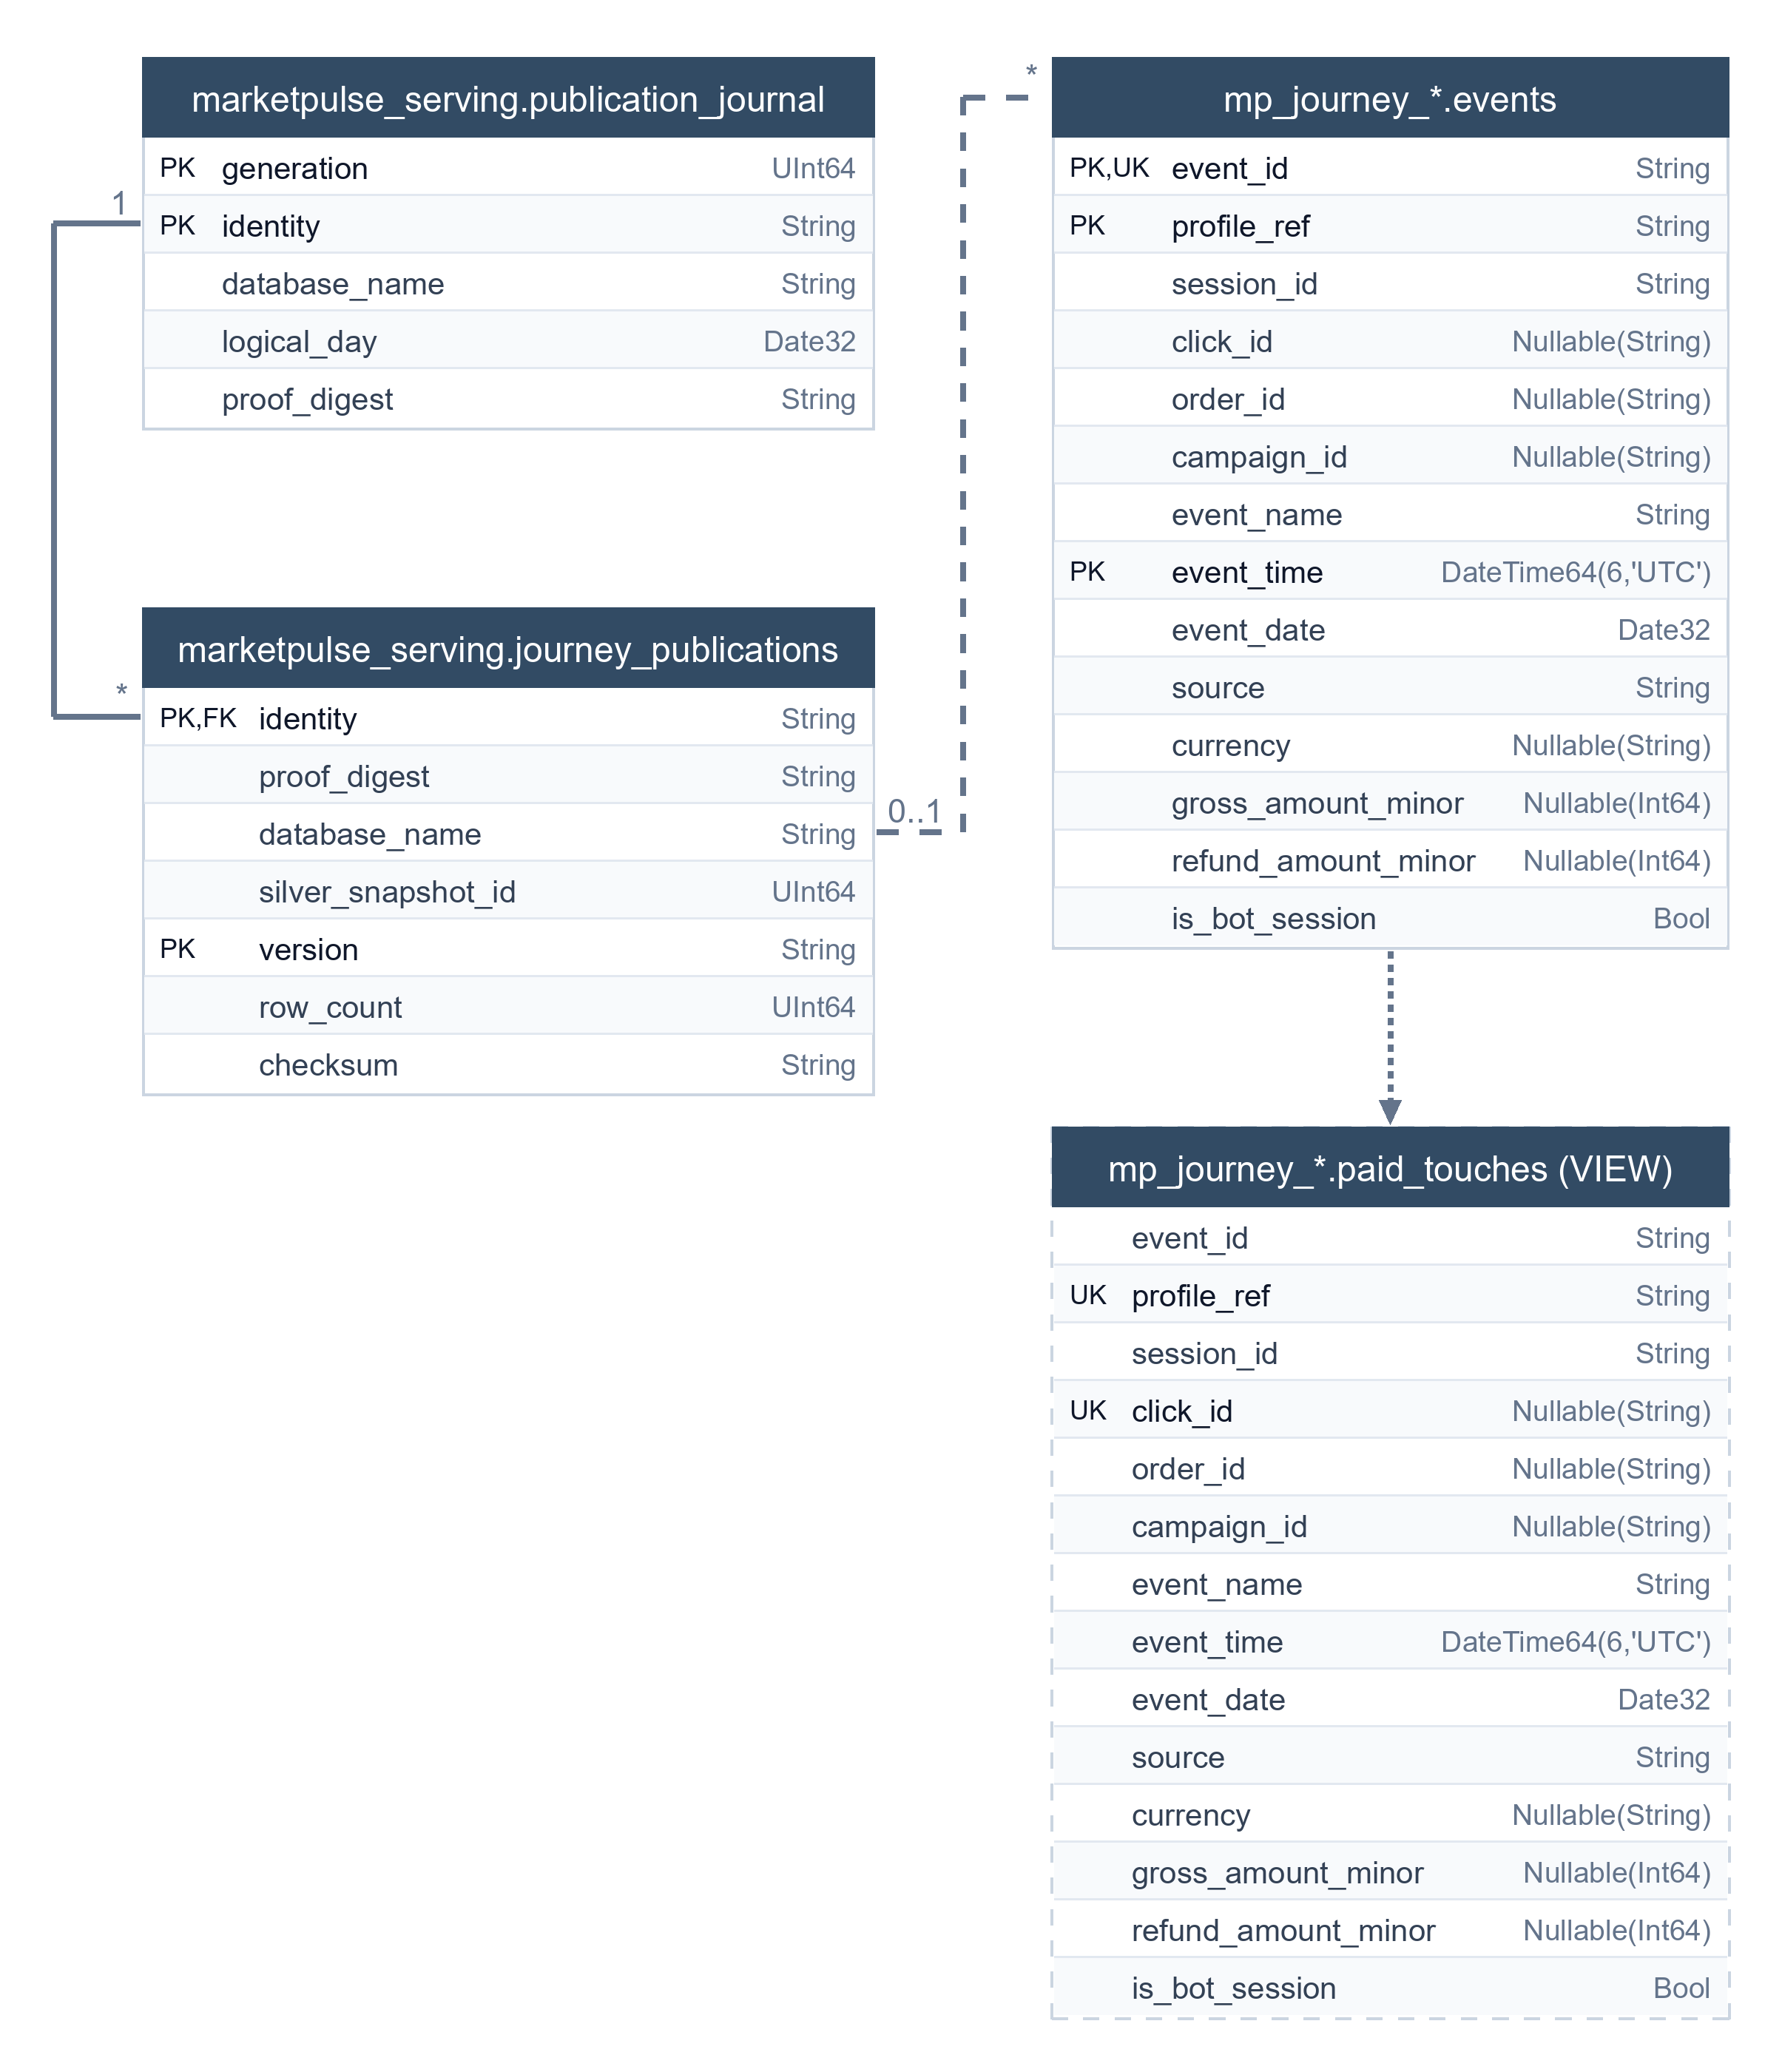
\includegraphics[width=\textwidth]{chapters/Pics/schema-clickhouse-1.png}
    \caption{Lược đồ quan hệ ClickHouse (phần 1): nhật ký công bố và CSDL hành trình (journey sidecar)}
    \label{fig:schema-clickhouse}
\end{figure}

\begin{figure}[!htbp]
    \centering
    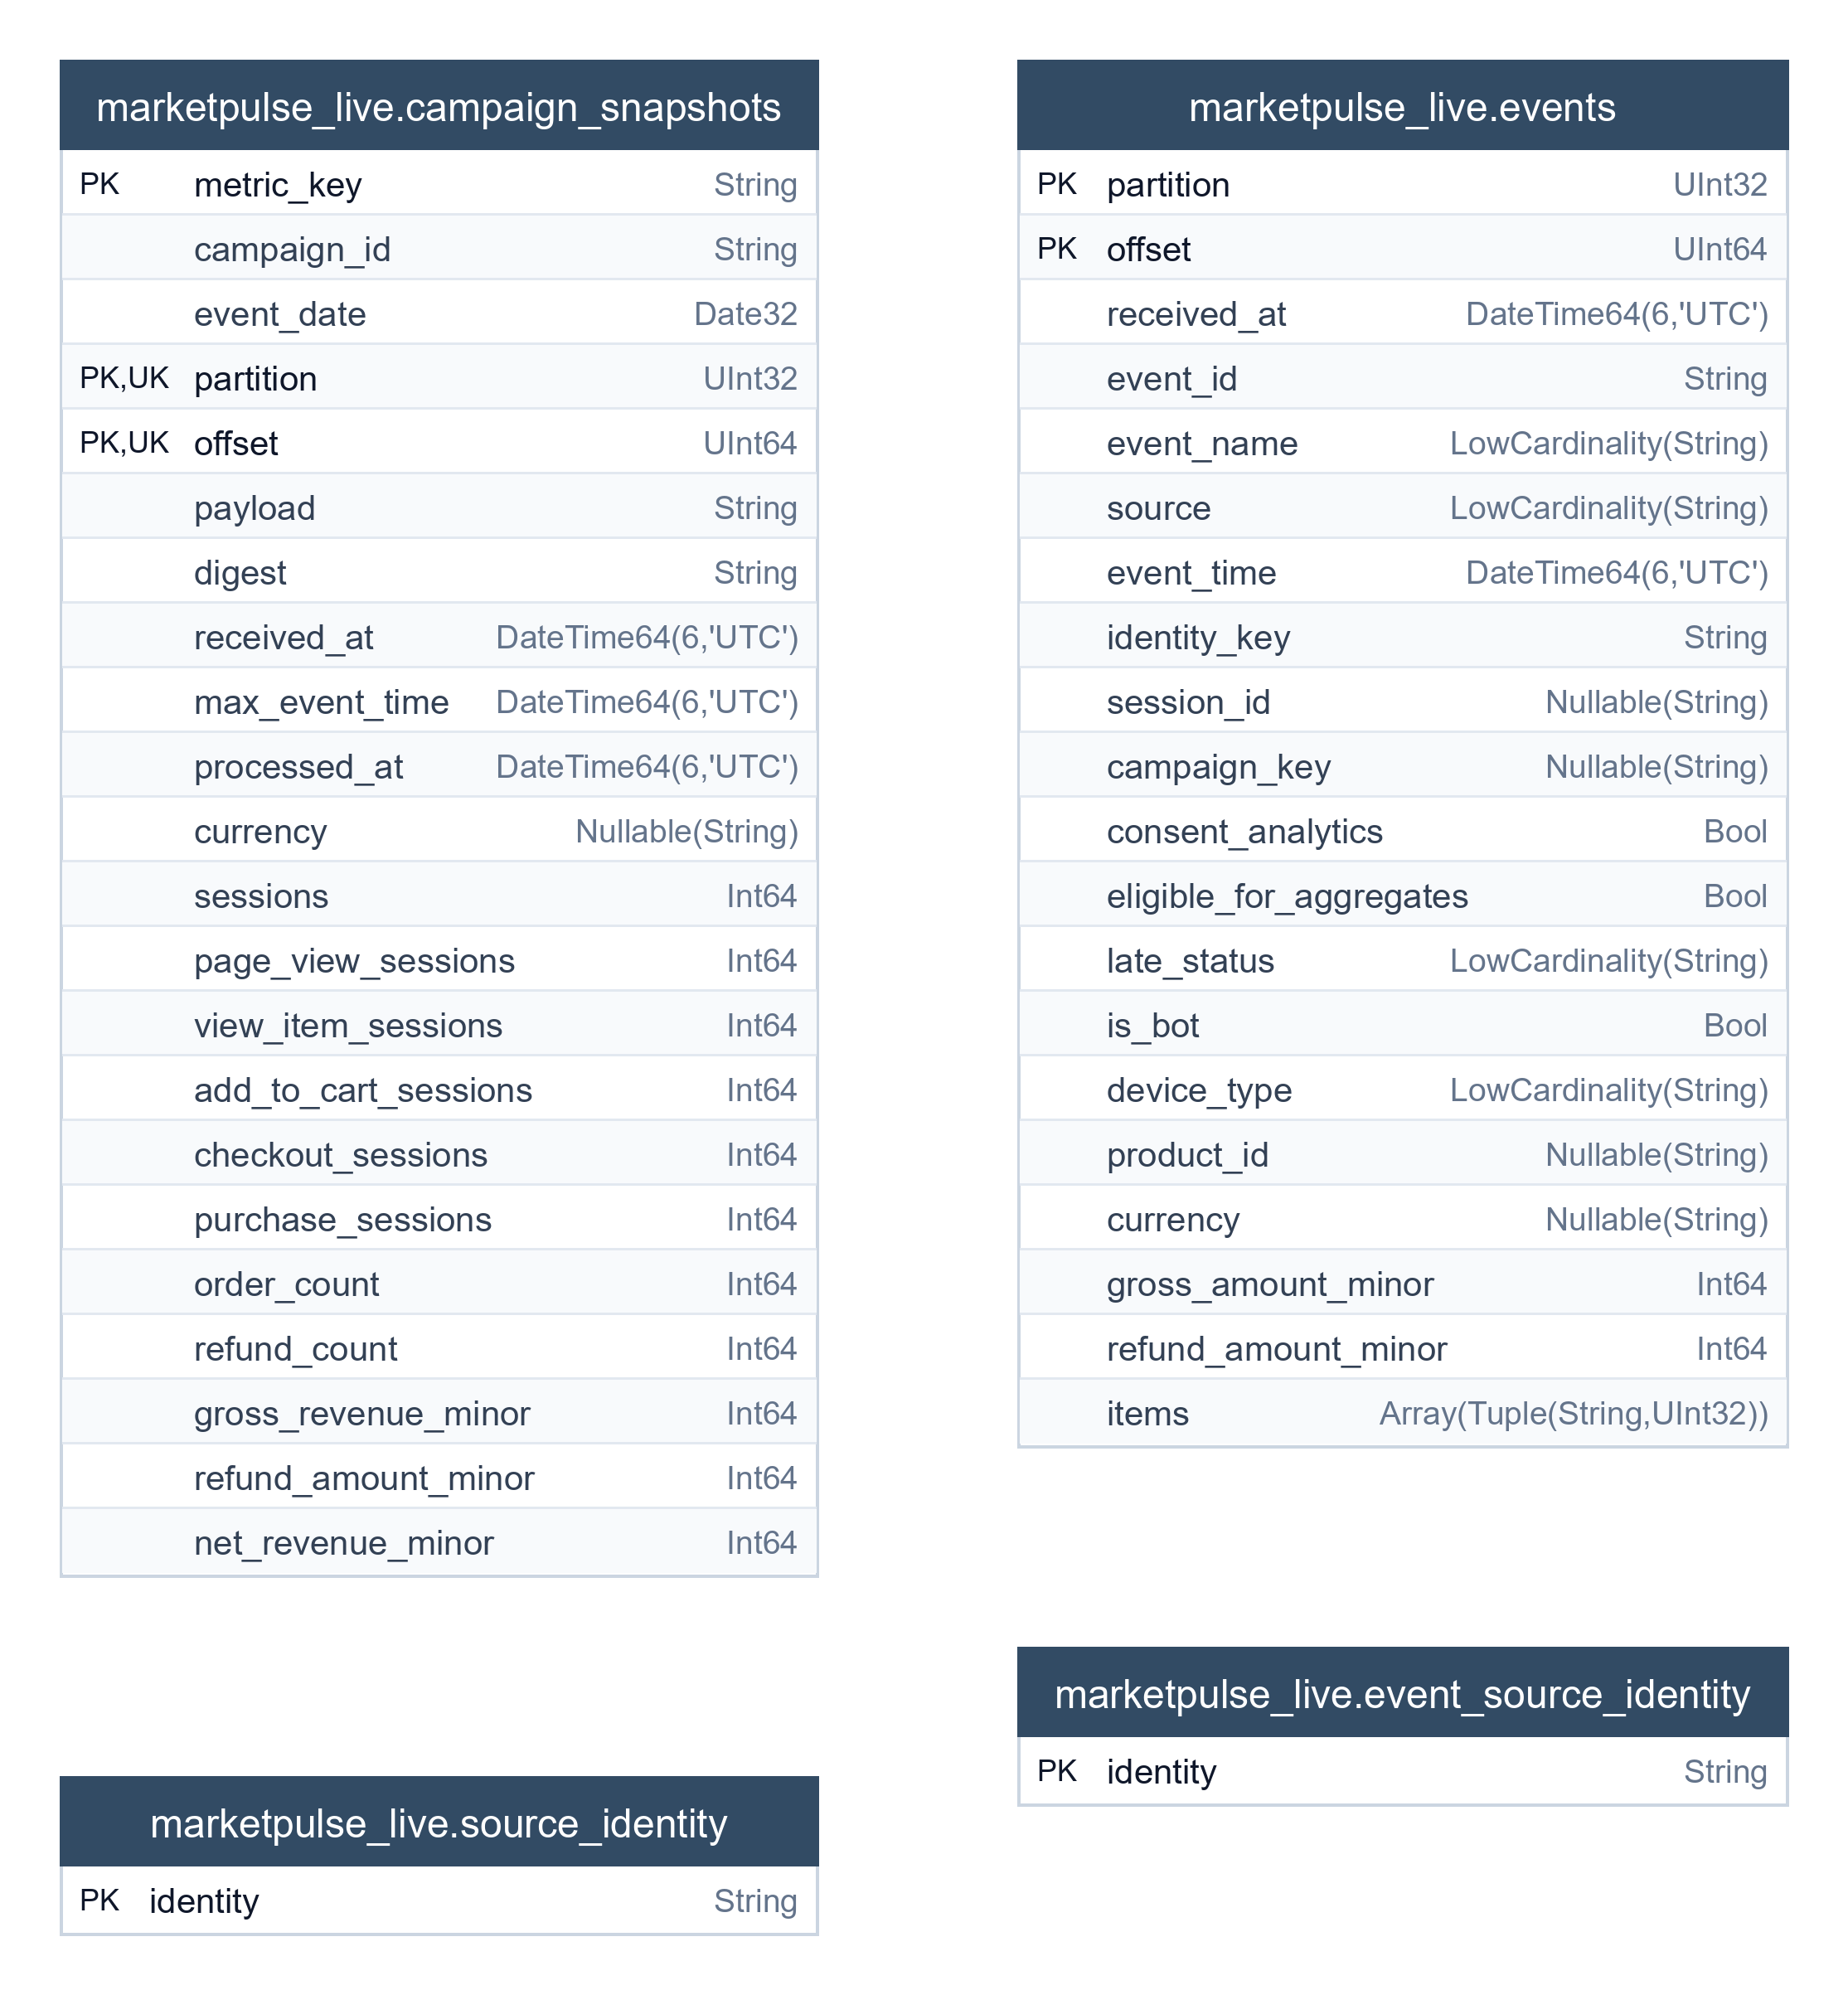
\includegraphics[width=0.92\textwidth]{chapters/Pics/schema-clickhouse-2.png}
    \caption{Lược đồ quan hệ ClickHouse (phần 2): kho dữ liệu trực tiếp \texttt{marketpulse\_live}}
    \label{fig:schema-clickhouse-2}
\end{figure}

\section{Giao diện và yêu cầu nghiệp vụ}
\label{sec:c4-giao-dien}

Kết quả trong phần này được đo trên release \texttt{109a2372\ldots} của bộ dữ liệu story-demo, gồm lịch sử đã kiểm chứng từ 01/01/2025 đến 31/08/2026 và luồng trực tiếp của tháng 09/2026. Mọi con số tổng hợp đều đã được một oracle độc lập tính lại từ file nguồn và khớp hoàn toàn (Mục~\ref{sec:c5-oracle}).

\subsection{Tổng quan giao diện}
\label{sec:c4-tong-quan-ui}
Giao diện được tổ chức thành 10 không gian làm việc, mỗi không gian phục vụ một nhóm câu hỏi (Bảng~\ref{tab:workspaces}). Nguyên tắc thiết kế xuyên suốt là \emph{trung thực về dữ liệu}: số liệu trực tiếp được gắn nhãn tạm thời và không bao giờ cộng với số liệu đã kiểm chứng; khi thiếu dữ liệu, giao diện hiển thị ``không có dữ liệu'' thay vì số 0; ngày tháng ghi rõ múi giờ.

\begin{table}[H]
\centering
\caption{Các không gian làm việc của Marketing Command Center}
\label{tab:workspaces}
\small
\renewcommand{\arraystretch}{1.2}
\begin{tabularx}{\textwidth}{>{\raggedright\arraybackslash}p{3.0cm} >{\raggedright\arraybackslash}p{2.2cm} >{\raggedright\arraybackslash}X}
\toprule
\textbf{Không gian} & \textbf{Đường dẫn} & \textbf{Nội dung chính} \\
\midrule
Overview & \texttt{/} & KPI chiến dịch đã kiểm chứng, số liệu trực tiếp, cảnh báo, giải ngân, mô phỏng \\
Live View & \texttt{/live} & Khách truy cập, phiên, đơn hàng của ngày hiện tại từ luồng trực tiếp \\
Ad Performance & \texttt{/ads} & Chi phí, click, ROAS theo nền tảng và chiến dịch \\
Analysis & \texttt{/analysis} & Phễu chuyển đổi, so sánh mô hình phân bổ, hành trình mẫu \\
Customers & \texttt{/customers} & Customer 360, dòng thời gian, phân đoạn, cohort, cơ hội và rủi ro \\
Email & \texttt{/email} & Số email đã gửi, đã nhận, được mở, được click, số lượt hủy đăng ký, số người nhận, tỷ lệ mở và click theo tháng \\
Insights & \texttt{/insights} & Nhịp hoạt động theo giờ, giá trị đơn hàng, kênh, khách hàng trung thành \\
Products & \texttt{/products} & Doanh thu theo ngành hàng và thiết bị \\
Geography & \texttt{/geography} & Doanh thu ròng theo 13 tỉnh/thành phố trên bản đồ Việt Nam \\
Data Health & \texttt{/operations} & Sức khỏe hệ thống, kiểm chứng chất lượng, lineage, kiểm toán \\
\bottomrule
\end{tabularx}
\end{table}

% Gợi ý: chèn ảnh chụp màn hình thật của từng không gian làm việc tại đây khi chạy story-demo, ví dụ:
% \begin{figure}[H]
%     \centering
%     \includegraphics[width=\textwidth]{chapters/Pics/ui-overview.png}
%     \caption{Màn hình Overview của Marketing Command Center}
%     \label{fig:ui-overview}
% \end{figure}

\subsection{Phân bổ doanh thu (BR-01)}
\label{sec:c4-br01}
Trong 20 tháng lịch sử, bốn nền tảng ghi nhận \num{2614669} lượt hiển thị, \num{227830} click và tổng chi phí \num{1339776177}~VND. Hình~\ref{fig:channels} đặt cạnh nhau tỷ trọng chi phí và tỷ trọng doanh thu gộp của từng nền tảng. Doanh thu ở đây được ghi nhận theo chiến dịch của click quảng cáo trả phí gắn trên chính đơn hàng (click của phiên mua hàng, hoặc click trả phí gần nhất trong 7 ngày trước đó), không theo mô hình First-Touch, Last-Touch hay Linear. Bốn nền tảng được ghi nhận tổng cộng \num{65,20}~tỷ VND trên \num{29059} đơn; \num{8,29}~tỷ VND còn lại (11,3\% doanh thu gộp, \num{3715} đơn) thuộc các đơn không có click trả phí nào trong 7 ngày trước khi mua nên không gắn với nền tảng nào. Shopee Ads chỉ chiếm 18,7\% chi phí nhưng mang về 31,5\% doanh thu gộp (\num{20,54}~tỷ VND từ \num{9158} đơn), trong khi Google Ads chiếm tỷ trọng chi phí lớn nhất (29,7\%) nhưng chỉ đóng góp 22,5\% doanh thu. Đây chính là loại phát hiện mà báo cáo riêng của từng nền tảng không thể đưa ra, và là cơ sở để \shCMO{} xem xét chuyển ngân sách. Trước khi quyết định, màn hình Analysis cho phép xem cùng phần doanh thu này được ba mô hình phân bổ ghi nhận khác nhau ra sao.

\begin{figure}[H]
\centering
\begin{tikzpicture}
\begin{axis}[
    name=left, xbar, width=0.43\textwidth, height=5.2cm, bar width=9pt,
    xmin=0, xmax=36, xlabel={Tỷ trọng chi phí (\%)},
    ytick={1,2,3,4}, yticklabels={Shopee,TikTok,Meta,Google}, 
    nodes near coords, nodes near coords align={horizontal},
    every node near coord/.append style={font=\scriptsize},
    tick label style={font=\footnotesize}, label style={font=\footnotesize},
    axis x line*=bottom, axis y line*=left, enlarge y limits=0.2]
  \addplot[fill=mphead, draw=mphead] coordinates {(29.7,4) (27.8,3) (23.8,2) (18.7,1)};
\end{axis}
\begin{axis}[
    at={(left.east)}, anchor=west, xshift=1.6cm,
    xbar, width=0.43\textwidth, height=5.2cm, bar width=9pt,
    xmin=0, xmax=36, xlabel={Tỷ trọng doanh thu gộp (\%)},
    ytick={1,2,3,4}, yticklabels={Shopee,TikTok,Meta,Google},
    nodes near coords, nodes near coords align={horizontal},
    every node near coord/.append style={font=\scriptsize},
    tick label style={font=\footnotesize}, label style={font=\footnotesize},
    axis x line*=bottom, axis y line*=left, enlarge y limits=0.2]
  \addplot[fill=mpaccent, draw=mpline] coordinates {(22.5,4) (25.6,3) (20.5,2) (31.5,1)};
\end{axis}
\end{tikzpicture}
\caption[Tỷ trọng chi phí và tỷ trọng doanh thu gộp theo nền tảng quảng cáo]{Tỷ trọng chi phí và tỷ trọng doanh thu gộp theo nền tảng quảng cáo, 01/2025 đến 08/2026. Doanh thu ghi nhận theo click trả phí gắn trên đơn hàng; mẫu số là \num{65,20}~tỷ VND doanh thu của bốn nền tảng}
\label{fig:channels}
\end{figure}

\subsection{Giám sát, cảnh báo và ngân sách (BR-02 -- BR-05)}
\label{sec:c4-br02-05}
Trong khi lịch sử dừng ở 31/08/2026, luồng tháng 09/2026 tiếp tục chảy vào màn hình Live View. Để kiểm tra số liệu trực tiếp có đáng tin hay không, nhóm đối chiếu màn hình với file nguồn tại cùng thời điểm phát lại (Bảng~\ref{tab:live-check}): sau khi khử trùng, lọc đồng thuận và loại phiên bot, hai bên khớp tuyệt đối.

\begin{table}[H]
\centering
\caption{Đối chiếu Live View với file nguồn tại thời điểm phát lại}
\label{tab:live-check}
\small
\renewcommand{\arraystretch}{1.2}
\begin{tabular}{lrr}
\toprule
\textbf{Chỉ số} & \textbf{Live View} & \textbf{File nguồn} \\
\midrule
Khách truy cập trong 30 phút gần nhất & 8 & 8 \\
Khách truy cập / phiên trong ngày & 224 / 231 & 224 / 231 \\
Đơn hàng & 25 & 25 \\
Doanh thu gộp (VND) & \num{60324000} & \num{60324000} \\
Hoàn tiền (VND) & \num{6805000} & \num{6805000} \\
Doanh thu ròng (VND) & \num{53519000} & \num{53519000} \\
\bottomrule
\end{tabular}
\end{table}

Cảnh báo (BR-03), giải ngân (BR-04) và mô phỏng (BR-05) cố ý dựa trên số liệu đã kiểm chứng của \texttt{campaign\_performance\_daily}, vì chi phí quảng cáo chỉ có ở nhánh lô. Ba loại quy tắc được hỗ trợ là vượt ngân sách, chi phí tăng đột biến so với ngày trước và tỷ trọng hoàn tiền; mỗi lần cảnh báo lưu kèm toán hạng, ngưỡng, cửa sổ thời gian và mã release làm bằng chứng. Phép mô phỏng tính doanh thu ròng dự kiến theo ROAS ròng lịch sử của từng chiến dịch và ghi rõ giả định ``kịch bản tuyến tính, không phải dự báo''.

\subsection{Kiểm chứng và sức khỏe hệ thống (BR-06)}
\label{sec:c4-br06}
Màn hình Data Health cho quản trị viên thấy release đang phục vụ, lineage từ snapshot Bronze đến \texttt{proof\_digest}, kết quả kiểm chứng lại toàn bộ bảng và đối soát tài chính, cùng nút chạy thử nghiệm làm hỏng có kiểm soát đã mô tả ở Ví dụ~4. Trên release story-demo, tổng doanh thu gộp \num{73488628000}~VND và hoàn tiền \num{4329091000}~VND khớp nhau giữa \texttt{commerce\_daily} và \texttt{campaign\_performance\_daily}, cho doanh thu ròng \num{69159537000}~VND trên \num{32774} đơn hàng.

\subsection{Phễu, Customer 360 và cohort (BR-07 -- BR-09)}
\label{sec:c4-br07-09}
Lớp hành trình gồm \num{298032} phiên web/app không phải bot. Kênh web có \num{198995} phiên với tỷ lệ chuyển đổi 11,9\%, ứng dụng có \num{99037} phiên với 8,5\%. Lưu lượng từ quảng cáo trả phí chiếm phần lớn (\num{219770} phiên xem trang), phần còn lại đến từ tìm kiếm tự nhiên, truy cập trực tiếp và email, chiếm 26,3\% số phiên sau quản trị. Nhịp hoạt động theo giờ Việt Nam cho thấy khung 20:00--22:00 có số phiên gấp 12,5 lần khung 02:00--04:00, cao điểm vào 21:00 thứ Bảy. Đây là thông tin hữu ích để lên lịch gửi email và chạy quảng cáo. Giá trị đơn hàng có trung vị \num{1797000}~VND và phân vị 90 là \num{4497000}~VND.

Ở góc độ sản phẩm (Hình~\ref{fig:products}), Thể thao và Làm đẹp dẫn đầu doanh thu gộp; máy tính để bàn và máy tính bảng tạo ra phần lớn doanh thu dù lưu lượng di động không nhỏ. Màn hình Customers cung cấp \num{748} dòng cohort theo tháng (các cohort từ 2023 đến 2026), hồ sơ Customer 360 với dòng thời gian hoạt động, phân đoạn RFM có lưu phiên bản và danh sách cơ hội như khách có nguy cơ rời bỏ (đã mua nhưng không quay lại từ 30 ngày) hoặc khách bỏ giỏ hàng.

\begin{figure}[H]
\centering
\begin{tikzpicture}
\begin{axis}[
    name=cat, xbar, width=0.43\textwidth, height=5.4cm, bar width=8pt,
    xmin=0, xmax=21, xlabel={Doanh thu gộp theo ngành hàng (tỷ VND)},
    ytick={1,2,3,4,5}, yticklabels={Thời trang,Gia dụng,Điện tử,Làm đẹp,Thể thao}, 
    nodes near coords, nodes near coords align={horizontal},
    every node near coord/.append style={font=\scriptsize},
    tick label style={font=\footnotesize}, label style={font=\footnotesize},
    axis x line*=bottom, axis y line*=left, enlarge y limits=0.15]
  \addplot[fill=mphead, draw=mphead] coordinates {(17.02,5) (16.74,4) (14.67,3) (12.90,2) (12.16,1)};
\end{axis}
\begin{axis}[
    at={(cat.east)}, anchor=west, xshift=1.9cm,
    xbar, width=0.43\textwidth, height=5.4cm, bar width=8pt,
    xmin=0, xmax=36, xlabel={Doanh thu gộp theo thiết bị (tỷ VND)},
    ytick={1,2,3,4}, yticklabels={Không rõ,Di động,Máy tính bảng,Máy tính}, 
    nodes near coords, nodes near coords align={horizontal},
    every node near coord/.append style={font=\scriptsize},
    tick label style={font=\footnotesize}, label style={font=\footnotesize},
    axis x line*=bottom, axis y line*=left, enlarge y limits=0.2]
  \addplot[fill=mpaccent, draw=mpline] coordinates {(29.45,4) (23.76,3) (18.94,2) (1.34,1)};
\end{axis}
\end{tikzpicture}
\caption{Doanh thu gộp đã kiểm chứng theo ngành hàng và theo thiết bị mua hàng}
\label{fig:products}
\end{figure}

Về địa lý (Hình~\ref{fig:geography}), TP.~Hồ Chí Minh và Hà Nội chiếm lần lượt 26,8\% và 25,0\% doanh thu ròng đã xác định vị trí. Khoảng \num{21,17}~tỷ VND đến từ hồ sơ ẩn danh hoặc chưa khớp được với khách hàng nên được tách riêng thành ``không xác định'' thay vì gán ngẫu nhiên cho một tỉnh thành; tổng các phần vẫn bằng đúng doanh thu ròng của Gold.

\begin{figure}[H]
\centering
\begin{tikzpicture}
\begin{axis}[
    xbar, width=0.82\textwidth, height=8.2cm, bar width=7pt,
    xmin=0, xmax=15, xlabel={Doanh thu ròng (tỷ VND)},
    ytick={1,2,3,4,5,6,7,8,9,10,11,12,13}, yticklabels={Hạ Long,Quy Nhơn,Huế,Buôn Ma Thuột,Vũng Tàu,Nha Trang,Hải Phòng,Biên Hòa,Đà Nẵng,Cần Thơ,Thủ Dầu Một,Hà Nội,TP. Hồ Chí Minh},
    nodes near coords, nodes near coords align={horizontal},
    every node near coord/.append style={font=\scriptsize},
    tick label style={font=\footnotesize}, label style={font=\footnotesize},
    axis x line*=bottom, axis y line*=left, enlarge y limits=0.05]
  \addplot[fill=mphead, draw=mphead] coordinates {
    (12.88,13) (12.02,12) (3.26,11) (2.82,10) (2.79,9)
    (2.74,8) (2.64,7) (1.77,6) (1.72,5) (1.42,4)
    (1.39,3) (1.36,2) (1.21,1)};
\end{axis}
\end{tikzpicture}
\caption{Doanh thu ròng đã kiểm chứng theo 13 tỉnh/thành phố (khách hàng đã xác định vị trí)}
\label{fig:geography}
\end{figure}

\subsection{Quyền riêng tư và tính lại lịch sử (BR-10)}
\label{sec:c4-br10}
Quản trị dữ liệu thể hiện trực tiếp trên số liệu: \num{1084} đơn hàng của khách từ chối đồng thuận phân tích không xuất hiện trong bất kỳ màn hình đã kiểm chứng nào. Hồ sơ trên giao diện chỉ hiện bút danh \texttt{profile\_ref}; phân đoạn chỉ được đánh dấu có thể kích hoạt khi khách hàng có đồng thuận marketing. Người dùng \texttt{viewer} không thấy và không gọi được các thao tác chi tiết hay vận hành; mọi quyết định truy cập nằm trong nhật ký kiểm toán. Việc tính lại lịch sử chạy cô lập qua \texttt{historical\_rebuild\_job} (Ví dụ~5) và không thay đổi release đang phục vụ.

\subsection{Tổng hợp đối chiếu yêu cầu}
\label{sec:c4-doi-chieu}
Bảng~\ref{tab:br-trace} truy vết mỗi yêu cầu nghiệp vụ tới màn hình, API và dữ liệu đã hiện thực.

\begin{table}[!htbp]
\centering
\caption{Truy vết yêu cầu nghiệp vụ tới màn hình, API (tiền tố \texttt{/api/v1}) và dữ liệu}
\label{tab:br-trace}
\footnotesize
\renewcommand{\arraystretch}{1.2}
\begin{tabularx}{\textwidth}{>{\raggedright\arraybackslash}p{1.1cm} >{\raggedright\arraybackslash}p{2.1cm} >{\raggedright\arraybackslash}p{6.0cm} >{\raggedright\arraybackslash}X}
\toprule
\textbf{BR} & \textbf{Màn hình} & \textbf{API chính} & \textbf{Dữ liệu} \\
\midrule
BR-01 & Analysis\newline Ads & \texttt{GET /analysis/attribution}\newline \texttt{GET /analysis/journeys} & \texttt{attribution\_daily}\newline \texttt{campaign\_performance\_daily}\newline \texttt{paid\_touches} \\
BR-02 & Overview\newline Live & \texttt{GET /dashboard}\newline \texttt{GET /live/view} & \texttt{marketpulse\_live.*} \\
BR-03 & Overview & \texttt{GET/POST /alert-rules}\newline \texttt{POST /alerts/evaluate} & \texttt{campaign\_performance\_daily}\newline bảng cảnh báo PostgreSQL \\
BR-04 & Overview & \texttt{GET /budget-pacing/\{campaign\_id\}} & \texttt{campaign\_settings}\newline \texttt{campaign\_performance\_daily} \\
BR-05 & Overview & \texttt{POST /budget-simulation} & \texttt{campaign\_performance\_daily} \\
BR-06 & Data Health & \texttt{POST /ops/quality/check}\newline \texttt{POST /ops/quality/probe} & release, \texttt{certified\_bundles}\newline \texttt{quality\_reports} \\
BR-07 & Analysis & \texttt{GET /analysis/funnel} & \texttt{funnel\_daily} \\
BR-08 & Customers\newline Email\newline Insights & \texttt{GET /lifecycle/profiles}\newline \texttt{GET /lifecycle/segments}\newline \texttt{GET /lifecycle/email-engagement}\newline \texttt{GET /insights/activity} & \texttt{customer\_360}\newline \texttt{mp\_journey\_*.events}\newline \texttt{segment\_revisions} \\
BR-09 & Customers\newline Products\newline Geography & \texttt{GET /lifecycle/cohorts}\newline \texttt{GET /insights/products}\newline \texttt{GET /insights/geography} & \texttt{cohort\_retention}\newline \texttt{commerce\_daily}\newline \texttt{customers} \\
BR-10 & Toàn bộ & \texttt{POST /auth/login}\newline \texttt{PUT /ops/users/\{id\}} & \texttt{auth\_*}, \texttt{access\_audit}\newline Silver đã quản trị \\
\bottomrule
\end{tabularx}
\end{table}
